\section{Experimental results}
\label{sec:experimental-results}

Our experimental evaluation was carried out using two machines, both running Linux and connected
using FDR InfiniBand. The first machine has each node
with 2 NVIDIA P100 GPUs, 2 Intel Broadwell E5-2683 v4, and 128GB for RAM. The second machine is 
equipped with 8 NVIDIA V100 and 2 Intel Xeon Gold 6148 per node. In 
both cases we are limited to use 4 nodes by the system scheduler. We used a database 
with up to XX billion SIFT descriptors, but
other descriptor, such as VLAD~\cite{jegou2010aggregating}, would also benefit from our optimizations. We used
OpenMPI version~2.1.2.

\subsection{IVFADC vs. FLANN and Exhaustive Exact k-NN}

The FLANN~\cite{Muja2009331, 6809191} implements several ANN algorithms, as described before,
and is able to choose the most efficient for a given database. As such, it is a good reference
for performance comparisons. Thus, here we compare IVFADC to FLANN to demonstrate its good quality
vs. speed tradeoff. The evaluation is performed on a SIFT database with 1 million descriptors and
10K queries by measuring the 1-recall@1, or the average proportion of the NNs ranked first in
the returned results, also referred to as precision~\cite{Muja2009331}. The experiments were
executed sequentially in the Intel Broadwell E5-2683 v4 CPU. The parameters of FLANN were
selected automatically, while we varied $w$ and the number of coarse centroids (shown as 
w/\# of centroids) in the graph. The same experiment was executed on the exact exhaustive k-NN  
using the Yael library, which employs BLAS/LAPACK underneath to attain high performance.
The exact k-NN took 1048.4 seconds, or about 0.1 second per query.


%The approach for approximate nearest neighbor search available in FLANN \cite{Muja2009331, 6809191} is known to be efficient. It employs hierarchical structures, i.e., using kd-trees and k-means trees, and can select the most efficient algorithm out of the choices available. It also tunes the algorithm’s parameters in a training phase to attain the best performance. An essential difference between FLANN and IVFADC/PQNNS is that the first maintains all vectors (descriptors) in RAM, because FLANN executes a re-ranking phase that computes the actual distance between the query vector and the candidate nearest neighbors. In PQANNS, on the other hand, only quantized values are kept in memory, reducing significantly the memory demands.
%
%The evaluation performed here presents the results for 1-recall@1, which is the average proportion nearest neighbors in the returned vectors or the precision. Although only R = 1 is used, the behavior of the methods is similar for larger values of R. The experiments were executed on a machine equipped with an 14-core Intel Haswell E5-2695, and both FLANN and IVFADC algorithms have indexed the dataset with 1M vectors and 10k query vectors. 
%
%The methods have been tuned to compare the search times for different quality results. The 
%FLANN parameters are chosen automatically by the tool, whereas for IVFADC the w and the number of %coarse centroids ( w /\# of centroids) were varied. For the sake of comparison, the same experiment %has also been executed for the exact algorithm that computes the k-NN using the Yael library. Yael is %an optimized library that implements the exact algorithm with functions from BLAS/LAPACK, which are %well known to be efficient. For reference, in that case, the experiment took about 1048.4 s.
\begin{figure}[htbp]
\centerline{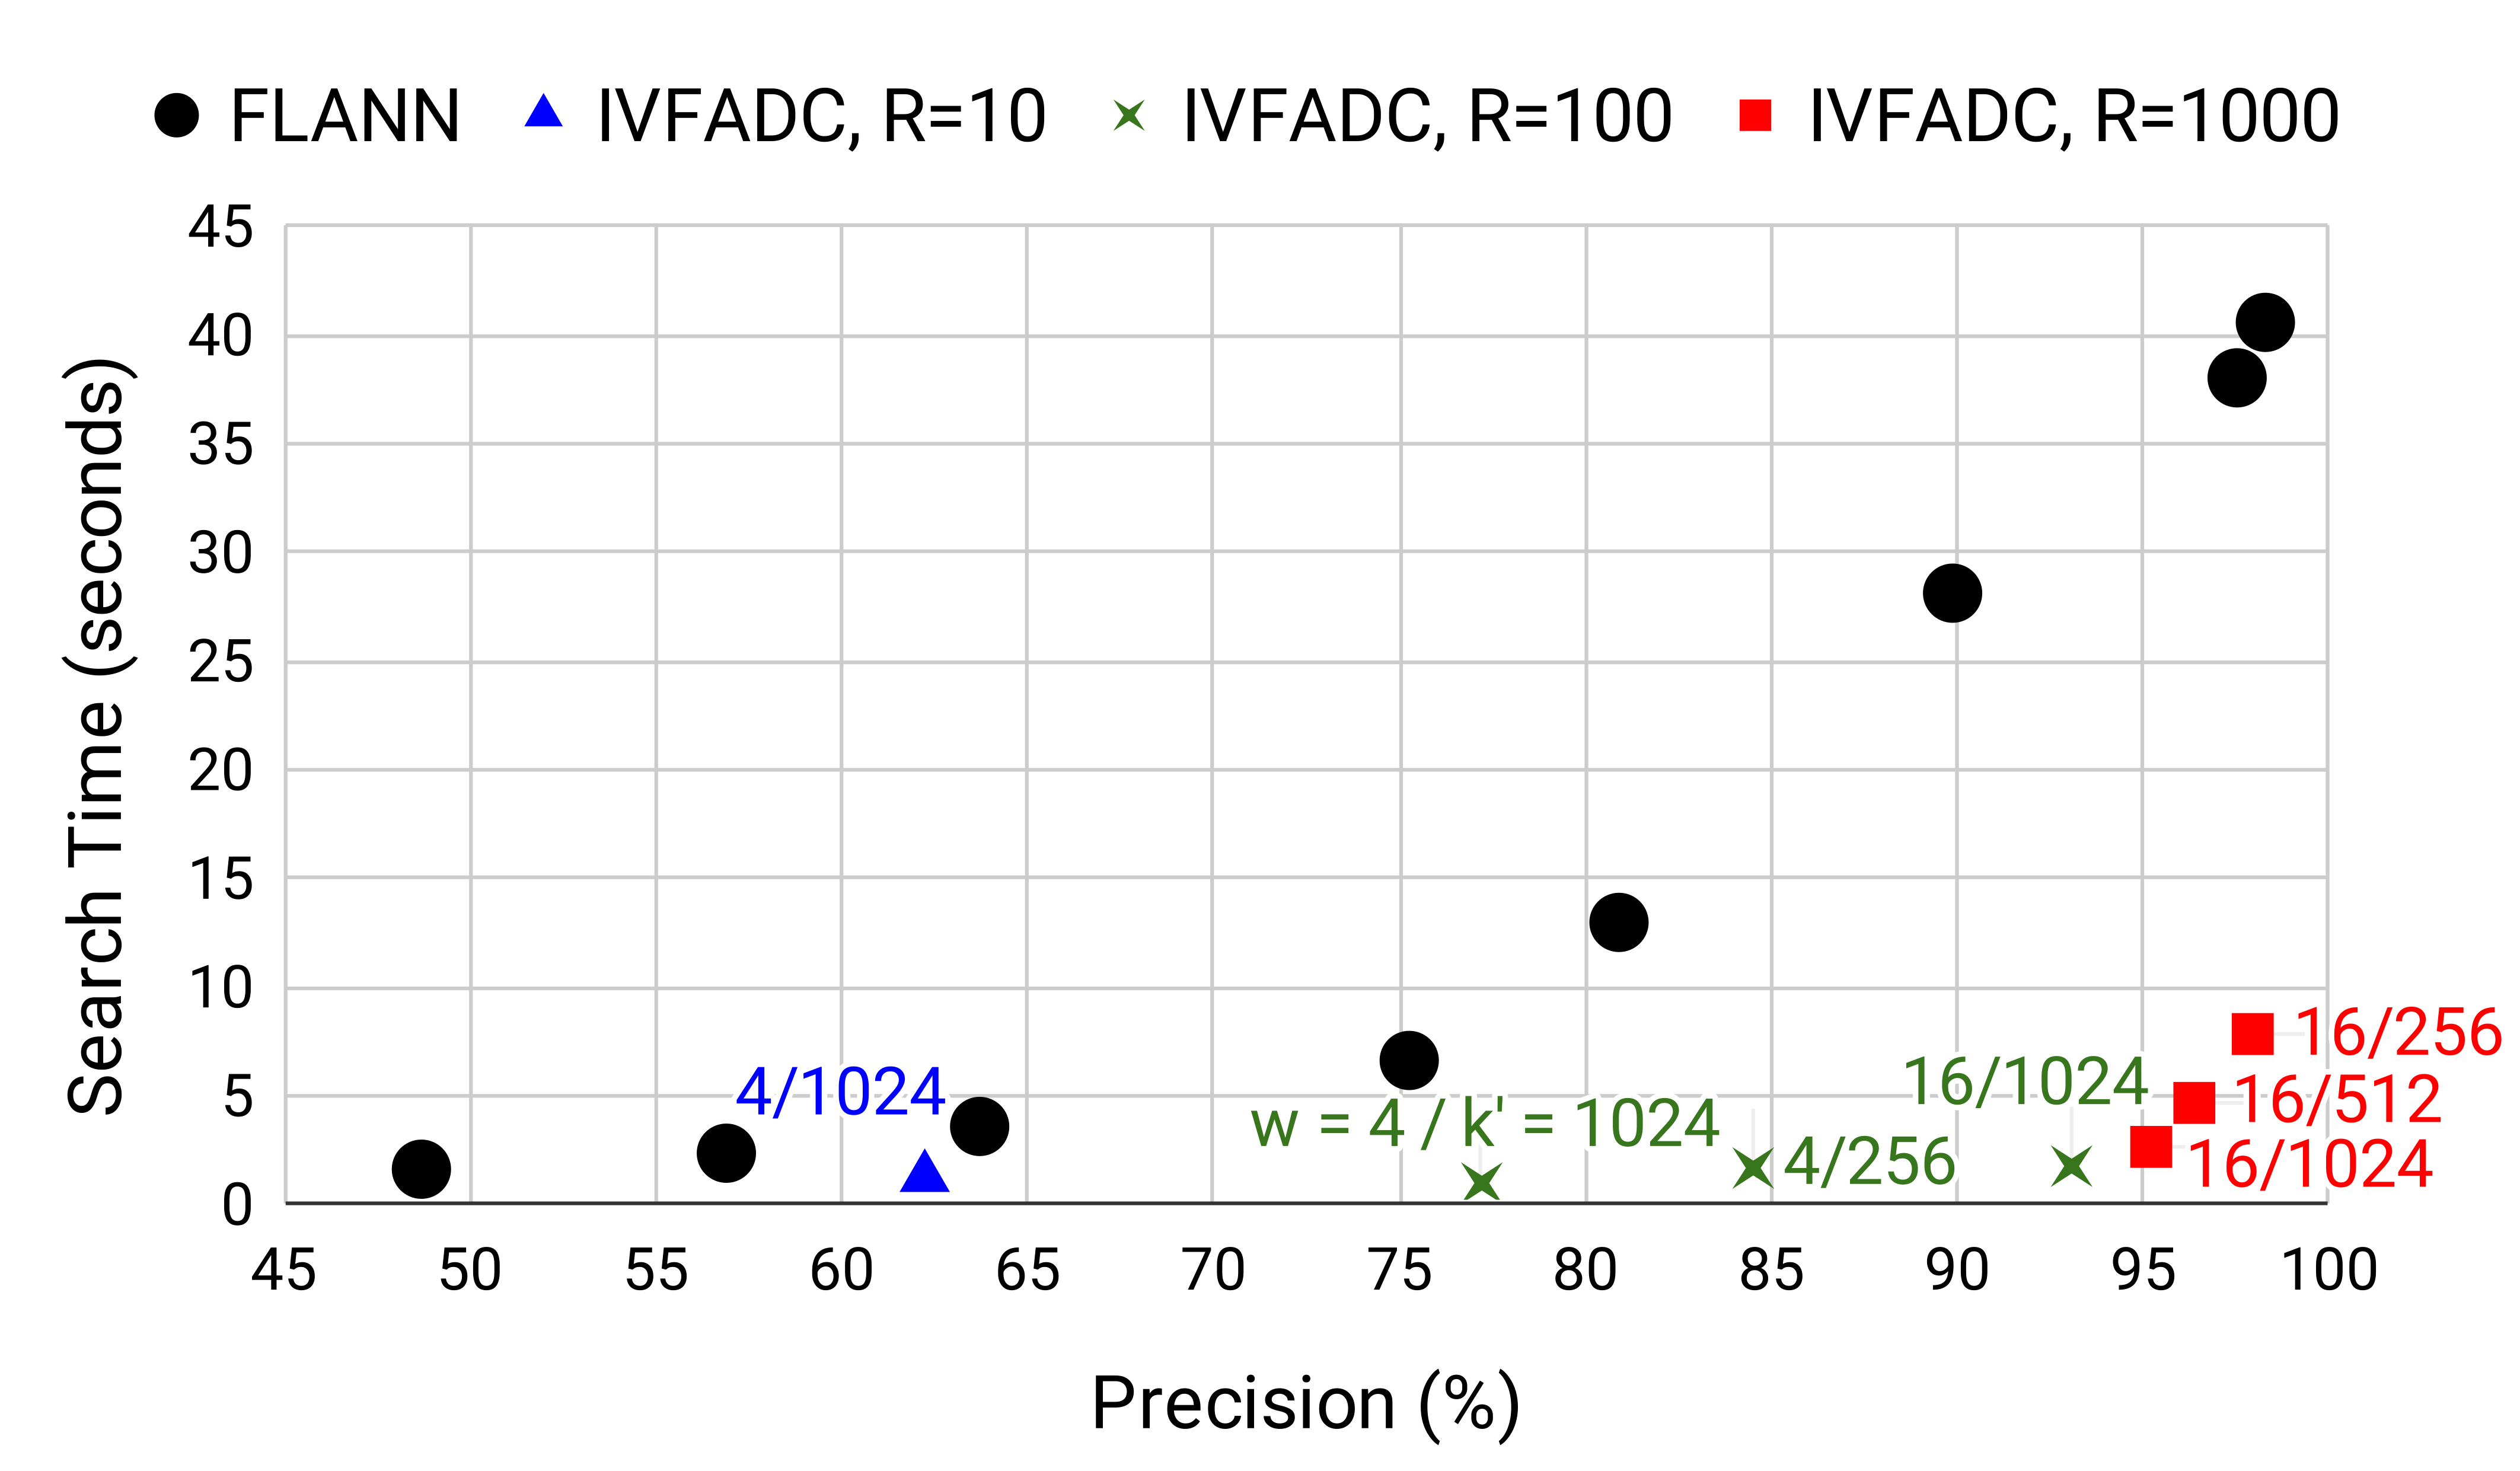
\includegraphics[width=\columnwidth]{figs/flann.png}}
\caption{IVFADC vs. FLANN: trade-offs between search quality (precision) and search time using CPU.}
\label{fig:flann}
\end{figure}

The results comparing IVFADC and FLANN as precision varies are shown in 
Figure~\ref{fig:flann}. As may be observed, for the same search quality,
IVFADC can execute significantly faster than FLANN, and their
performance gap increases with higher precision. It is also 
impressive that FLANN uses 600~MB of memory, whereas IVFADC needs only 26~MB. 
For 98\% precision, the amortized search 
time per query with IVFADC is less that 0,00078 sec or 127$\times$ faster
than the exact k-NN.


\subsection{The Performance of CPU, GPU, and CPU-GPU}
\label{sec:in-core-throughput}

This section presents the baseline single node throughput of our implementation 
on multi-core CPU, GPU, and cooperative CPU-GPU executions using the 
first machine. These experiments were executed with 500~million SIFT vectors 
and 100k queries, which were sent for execution at the beginning of the experiments. 
The IVFADC has been configured to use a coarse codebook with 4096 elements, m=8, and 256 
clusters per sub-dimension. This configuration attained a precision of 76\%.
%an average search precision of BB\%.  R@1000 = 0.9358


\begin{table}[htbp]
\caption{Throughput (queries/s) with different configs.}
\vspace{-4mm}
\begin{center}
\begin{tabular}{ccc}  
\hline
%\multicolumn{3}{c}{\textbf{System setup}} \\
\textbf{CPU only}        & \textbf{GPU only}      &   \textbf{CPU-GPU} \\ \hline \hline
 %\textbf{Setup}         & \textbf{Avg. Query Time}   & \textbf{Throughput (queries/s)} \\ \hline \hline
  799                    & 5635                   & 6364  \\ \hline
  %GPU Only              & 0.00001                   & 2481  \\ \hline
%  CPU + GPU             & 0.00001                   & 3894  \\ \hline
\end{tabular}
\label{tab:batch-throughput}
\end{center}
\end{table}

The performance is presented in Table~\ref{tab:batch-throughput} according
to the system configuration used in the LI phase of the parallel algorithm: 
CPU only, GPU only, or 
CPU-GPU. The CPU only execution employs the 28 CPU cores available, and 
the CPU-GPU maintains a copy of the index in each device and divides queries 
between CPU and GPU proportionally to their relative performance as 
detailed in Section~\ref{sec:intra-cooperative}. The query rate attained 
is very high in all cases with the GPU being about 7$\times$ faster than 
a 14 core CPU. The CPU-GPU execution in turn attains a speedup of 
1.12$\times$ on top of the GPU. The performance is slightly smaller than the sum 
of the processors throughput because (i)~a CPU core is reserved to manage 
the GPU; and, (ii)~there are inevitable overheads, including load imbalance, 
query partitioning, etc. 

\subsection{The Performance of GPU Out-of-core Execution}
\label{sec:out-of-core-throughput}

This section evaluates our out-of-core execution scheme with 
GPU only and CPU-GPU. It employs the same database and IVFADC configuration 
used in the previous section. However, for the sake of analyzing the out-of-core 
effects to the performance, the amount of data that may be kept in the GPU 
memory at any time during the execution is limited. Furthermore,
this amount is varied with purpose of analyzing multiple GPU memory 
capabilities and evaluate the performance in different scenarios.

\begin{table}[htbp]
\caption{Throughput (queries/s) in an out-of-core execution.}
\vspace{-4mm}
\begin{center}
\begin{tabular}{ccccc}  
\hline
\multirow{2}{*}{\textbf{\makecell{\% of data\\ in GPU}}} & \textbf{\makecell{GPU\\ only}} & \textbf{\makecell{CPU-GPU\\Fixed Division}}  &  \textbf{\makecell{CPU-GPU\\Work Stealing}}\\ 
                        &       &           &       \\ \hline \hline
12.5\%                  &   3422&  867     &  4061 \\ \hline
25\%                    &   4113&  1010     &  4908 \\ \hline
50\%                    &   4443&  1503     &  5607 \\ \hline
\end{tabular}
\label{tab:out-throughput}
\end{center}
\end{table}

The throughput of the system is presented in Table~\ref{tab:out-throughput}
as the percentage of the index that would fit in the GPU memory, from 12.5\% up to 50\%,  
 is varied. As shown, the GPU-only configuration attained significant performance
even in cases in which the amount of the index it can hold up is small (12.5\%) and,
as expected, its performance improves as more data is kept in memory. The GPU only
out-of-core execution reached a throughput of 80\% of the case in which
all the data fits in memory, presented in the previous section. Also, it is about 
5.56$\times$ faster than using only the CPU. 

%it is about 5.56$\times$ faster than
%using only the CPU and it attains close to 80\% of the performance of the execution
%with all data in memory. This is an important aspect in terms of determining
%the cost-benefit of buying or not the more expensive GPUs with larger memory capacity.
%GPUs with large memories, which tends to be
%far more expensive.

Further, it is presented the performance of the GPU-GPU execution with a fixed 
data division between CPU and GPU and using work stealing. In the fixed case, 
because the GPU can only process the index subpartition assigned to it, 
the CPU becomes the bottleneck and the cooperative execution is ineffective. 
However, the CPU-GPU with work stealing improved the GPU-only in all cases 
and attained a speedup of 1.26$\times$ for the case in which 50\% of data can
be stored in the GPU memory. As such, the appropriate cooperative execution 
has attained higher gains in the out-of-core case, which is a consequence
of having the GPU running slower due to the required CPU-GPU data transfers. Also,
with the CPU cooperation, the number of costly data transfers is significantly reduced vs
the GPU only case because they are only performed to steal subpartitions from 
the CPU in cases where the latter is overloaded.

\subsection{The Effect of Run-Time Optimizations to Response Time}

This section evaluates the effect of our optimization to the queries
response times under fluctuating workloads. The evaluations are
performed for the cases in which the data fits (in-core) and do not fit 
(out-of-core) into the GPU memory. The database with 500~million SIFT vectors 
and 100k queries has been used along with the same IVFADC setup
employed in Section~\ref{sec:in-core-throughput}. 

\subsubsection{In-Core GPU and CPU-GPU Execution}

We evaluate GPU and CPU-GPU execution with multiple strategies to
adapt the system (query block size) in on-line scenarios with fluctuating 
loads. Our DQPP policy (Section~\ref{sec:query-rate-aware}) is compared
to the Best Static (BS) and Dynamic Greedy Dispatch (DGD). BS uses
the static block size that leads to best average query response time in 
each load. This block size is selected by varying its value and selecting
the one with the best value. It is, however, unfeasible in practice since
one would not know in advance the load that it would experience. DGD is a dynamic
approach that calls the GPU execution for all queries available 
whenever the GPU becomes idle. Although DGD would be able to adapt to fluctuating workloads, it
does not include the smart mechanism of DQPP that also looks into
the near past to decide whether to call or not the GPU for a given queue size.
The fluctuating query workload is implemented using a Poisson distribution 
with expected average rate ($\lambda$) varying from 20\% (0.2) to 100\% (1.0) 
of the GPU throughput (queries/s) presented in Section~\ref{tab:out-throughput}.

\begin{table}[htbp]
\caption{Average query response time (secs.) with varying query rates using a Poisson distribution ($\lambda\ \times$ maximum throughput) for GPU only and CPU-GPU execution.}
\vspace{-4mm}
\begin{center}
\resizebox{\columnwidth}{!}{%
\begin{tabular}{c|ccc|ccc}  
  \hline
% \multirow{2}{*}{\textbf{\makecell{Poisson $\lambda$ (\% of\\ max. throughput)}}} & \multirow{2}{*}{\textbf{BS}} & \multirow{2}{*}{\textbf{DGD}} & \multirow{2}{*}{\textbf{DQPP}} \\  
\multirow{2}{*}{$\lambda$}   & \multicolumn{3}{c}{\textbf{GPU}}   & \multicolumn{3}{c}{\textbf{CPU-GPU}}  \\
            & \textbf{BS} & \textbf{DGD} & \textbf{DQPP} & \textbf{BS} & \textbf{DGD} & \textbf{DQPP} \\\hline \hline
  0.2       & 0.121  & 0.007  & 0.007   &    0.122       &    0.012     & 0.010 \\ \hline
  0.4       & 0.117  & 0.069  & 0.056   &    0.108       &    0.054     & 0.046\\ \hline
  0.6       & 0.180  & 0.221  & 0.139   &    0.154       &    0.160     & 0.114 \\ \hline
  0.8       & 0.363  & 1.132  & 0.359   &   0.260        &    0.426     & 0.235 \\ \hline
  1         & 0.872  & 2.406  & 0.897   &   0.590        &    1.312     & 0.575 \\ \hline
\end{tabular}
}
\label{tab:in-core-gpu-rt}
\end{center}
\end{table}



%\begin{table}[htbp]
%\caption{Average query response time (secs.) with varying query rates using a Poisson distribution ($\lambda\ \times$ maximum throughput) for GPU only and CPU-GPU execution.}
%\vspace{-4mm}
%\begin{center}
%\resizebox{\columnwidth}{!}{%
%\begin{tabular}{c|ccc|ccc}  
%  \hline
% \multirow{2}{*}{\textbf{\makecell{Poisson $\lambda$ (\% of\\ max. throughput)}}} & \multirow{2}{*}{\textbf{BS}} & \multirow{2}{*}{\textbf{DGD}} & \multirow{2}{*}{\textbf{DQPP}} \\  
%\multirow{2}{*}{$\lambda$}   & \multicolumn{3}{c}{\textbf{GPU}}   & %\multicolumn{3}{c}{\textbf{CPU-GPU}}  \\
 %           & \textbf{BS} & \textbf{DGD} & \textbf{DQPP} & \textbf{BS} & \textbf{DGD} & \textbf{DQPP} \\\hline \hline
%  0.2       & 0.121249  & 0.00718  & 0.007193    &    0.122482       &    0.012468       & 0.010728 \\ \hline
%  0.4       & 0.117798  & 0.069342  & 0.056245   &    0.108122       &    0.054811       & 0.046971\\ \hline
%  0.6       & 0.180421  & 0.221665  & 0.139796   &    0.154673       &  0.160175         & 0.114136 \\ \hline
%  0.8       & 0.363235  & 1.132886  & 0.359531   &   0.260399        &   0.426465        & 0.235068 \\ \hline
%  1         & 0.872433  & 2.406216  & 0.897363   &   0.590762        &   1.31214        & 0.575897 \\ \hline
%\end{tabular}
%}
%\label{tab:in-core-gpu-rt}
%\end{center}
%\end{table}

The average query response times of the strategies are presented in 
Table~\ref{tab:in-core-gpu-rt}. The BS and DGD comparison shows that
the first attains best results for high loads ($\lambda \geq 0.6$), whereas
the latter is faster for lower loads. Because BS will use a single block size,
it favors high load cases in which the response times are also higher because
improving that zone leads to better gains. The results also highlight that
a single block size will, in fact, not be the best choice.
%, and that DGD could
%not effectively take advantage of its ability to take the block size decision
%during the execution.

Further, the DQPP has improved DGD and BS for most of the configurations, showing
that it can perform well in all workload levels. As expected,
for higher loads, the DQPP will not be able to improve BS, because
the system is overloaded and the block size chosen by BS coincides with the one
that leads to the highest throughput. However, as with smaller $\lambda$ the load
effectively varies during the execution and DQPP will improve BS. For a $\lambda=0.6$, for
instance, DQPP has reduced the response times of BS in 1.29$\times$ and 1.35$\times$ 
for the GPU and CPU-GPU configurations, respectively.

\subsubsection{Out-of-Core GPU and CPU-GPU Execution} This evaluates
our out-of-core approach by varying the
amount of data (\% of the index) that fits in the GPU memory. The
results are presented in Table~\ref{tab:out-of-core-gpu-rt}, in which the 
CPU only execution is also included for reference.


%\begin{table}[htbp]
%\caption{Average query response time (secs.) with varying query rates using a Poisson distribution ($\lambda\ \times$ maximum throughput) for GPU only and CPU-GPU execution.}
%\vspace{-4mm}
%\begin{center}
%\resizebox{\columnwidth}{!}{%
%\begin{tabular}{c|c|cccc}  
%  \hline
%\textbf{Data in GPU}&   $\lambda$   & \textbf{CPU}  & \textbf{CPU-GPU Fixed} & \textbf{GPU}    & \textbf{CPU-GPU WS}   \\\hline \hline
%\multirow{5}{*}{\rot{\textbf{\makecell{50\%}}}}
%&  0.2       & 25.75656667          & 0.9807666667      & 6.975402      & 1.682377         \\ \cline{2-6}
%&  0.4       & 59.65157633         & 9.601725667      & 8.462452667      & 3.177517333     \\ \cline{2-6}
%&  0.6       & 76.58238          & 17.13314467      & 10.181424       & 3.608836667       \\ \cline{2-6}
%&  0.8       & 80.467399         & 21.01687433     & 11.434746      & 4.403954333        \\ \cline{2-6}
%&  1         & 95.28662233         & 23.354318      & 13.11479067      & 5.253602333      \\ \hline
%\multirow{5}{*}{\rot{\textbf{\makecell{25\%}}}}
%&  0.2       & 25.75656667      & 5.872821667  & 8.674977333      & 2.886341667        \\ \cline{2-6}
%&  0.4       & 59.65157633      & 25.53414133   & 10.47723267   & 4.426854667       \\ \cline{2-6}
%&  0.6       & 76.58238        & 33.13529133   & 11.413043     & 5.736826667        \\ \cline{2-6}
%&  0.8       & 80.467399         & 36.81468233   & 13.72247867     & 6.636542667          \\ \cline{2-6}
%&  1         & 95.28662233      & 39.17210033     & 13.54772167     & 7.749284        \\ \hline
%\multirow{5}{*}{\rot{\textbf{\makecell{12.5\%}}}}
%&  0.2       & 25.75656667      & 11.91608967   & 12.487547     & 4.707428       \\ \cline{2-6}
%&  0.4       & 59.65157633      & 33.61884467   & 14.88388267   & 6.914897         \\ \cline{2-6}
%&  0.6       & 80.467399        & 41.4779355    & 17.801245     & 8.6922205        \\ \cline{2-6}
%&  0.8       & 76.58238         & 45.061773     & 20.7138785    & 10.373042          \\ \cline{2-6}
%&  1         & 95.28662233      & 47.410779     & 20.796574     & 11.473293      \\ \hline
%\end{tabular}
%}
%\label{tab:out-of-core-gpu-rt}
%\end{center}
%\end{table}

TABLE COMENTADA, FIX THE CODE

%
%\begin{table}[htbp]
%\caption{Average query response time (secs.) with varying query rates using a Poisson distribution ($\lambda\ \times$ maximum throughput) for GPU only and CPU-GPU execution.}
%\vspace{-4mm}
%\begin{center}
%\resizebox{\columnwidth}{!}{%
%\begin{tabular}{c|c|ccc}  
%  \hline
%\multirow{2}{*}{\textbf{\makecell{\% of data\\ in GPU}}} &   \multirow{2}{*}{\textbf{\makecell{$\lambda$}}}   & \multirow{2}{*}{\textbf{\makecell{CPU\\ only}}}  & \multirow{2}{*}{\textbf{\makecell{GPU\\ only}}}  & \multirow{2}{*}{\textbf{\makecell{CPU-GPU\\ Fixed}}}   & \multirow{2}{*}{\textbf{\makecell{CPU-GPU\\ Work Stealing}}}   \\\hline \hline
%    &       &           &           &           & \\\hline \hline
%\multirow{5}{*}{\rot{\textbf{\makecell{12.5\%}}}}
%&  0.2       & 25.756   & 12.487    & 11.916    & 4.707       \\ \cline{2-6}
%&  0.4       & 59.651   & 14.883    & 33.618    & 6.914         \\ \cline{2-6}
%&  0.6       & 80.467   & 17.801    & 41.477    & 8.692        \\ \cline{2-6}
%&  0.8       & 76.582   & 20.713    & 45.061    & 10.373          \\ \cline{2-6}
%&  1         & 95.286   & 20.796    & 47.410    & 11.473      \\ \hline
%\multirow{5}{*}{\rot{\textbf{\makecell{25\%}}}}
%&  0.2       & 25.756   & 8.674     & 5.872     & 2.886        \\ \cline{2-6}
%&  0.4       & 59.651   & 10.477    & 25.534    & 4.426       \\ \cline{2-6}
%&  0.6       & 76.582   & 11.413    & 33.135    & 5.736        \\ \cline{2-6}
%&  0.8       & 80.467   & 13.722    & 36.814    & 6.636          \\ \cline{2-6}
%&  1         & 95.286   & 13.547    & 39.172    & 7.749        \\ \hline
%\multirow{5}{*}{\rot{\textbf{\makecell{50\%}}}}
%&  0.2       & 25.756   & 6.975     & 0.980     & 1.682         \\ \cline{2-6}
%&  0.4       & 59.651   & 8.462     & 9.601     & 3.177     \\ \cline{2-6}
%&  0.6       & 76.582   & 10.181    & 17.133    & 3.608       \\ \cline{2-6}
%&  0.8       & 80.467   & 11.434    & 21.016    & 4.403        \\ \cline{2-6}
%&  1         & 95.286   & 13.114    & 23.354    & 5.253      \\ \hline
%\end{tabular}
%}
%\label{tab:out-of-core-gpu-rt}
%\end{center}
%\end{table}

As presented, the average response times in the execution using only 
the CPU or GPU only are much higher as compared with GPU in-core data. Although
the GPU attains a good throughput in the out-of-core execution
(Section~\ref{sec:out-of-core-throughput}), because data transfers costs 
are amortized by the execution of several queries, this is
not the case for the response time. If a query needs to wait until, for instance, 50\%
of the data is transferred into the GPU for execution, that time will actually be
summed to the response time of each query waiting to be processed. This aspect also
explains why, although the CPU-GPU fixed throughput is smaller than the GPU-only, 
as presented in Table~\ref{tab:out-throughput}, it can attain better response times than
the GPU-only for low loads. It is impressive, for instance, that the CPU-GPU algorithm, fixed
for 50\% of the data in the GPU, was able to reduce the response times of the 
GPU-only in 7.11$\times$ for a load $\lambda=0.2$. As the load increases, however, this
is inverted because queue waiting becomes a bottleneck due to the low CPU throughput. 
Further, the response times improvements with the CPU-GPU using work stealing
are impressive. As compared to the GPU-only configuration, which attains better overall
response times than the CPU-GPU fixed, the CPU-GPU with work stealing reduced the
response times in about 2.4$\times$ on average. This approach attained reasonable response
times, even with high loads and a small percentage of the index in the GPU memory. 

\subsection{Distributed Memory Scalability}

